% ---------------------------------------------------------------------
% Das Dokument kompiliert mit pdflatex und ist auf Basis 
% von Koma-Script entstanden. 
%
% Autor des Templates (für Anmerkungen): 
% Michael von Riegen, riegen@informatik.uni-hamburg.de
%
% Einzelne Code-Teile für das Titelblatt sind aus dem Template 
% von Benjamin Kirchheim entnommen.
%
% 25.05.09, Frank Langanke: Vorlage auf aktuelle KOMA-Version aktualisiert
% 26.05.09, Michael von Riegen: Anmerkung --> aktuelles Koma-Script ist nötig!
% 17.10.2016 neues Uni logo
% ---------------------------------------------------------------------
\documentclass[11pt,DIV=15,BCOR=20mm,bibliography=totoc]{scrbook}

% Import von Paketen und Optionen die das gesamte Dokument betreffen
% sind in myPreamble.sty ausgelagert.
\usepackage{_preamble}
\usepackage{graphicx} % Required for inserting images
\usepackage{subcaption}
\usepackage[
backend=biber,
style=alphabetic,
]{biblatex}
\usepackage[utf8]{inputenc}
\usepackage{listings}
\usepackage{pgfplots}
\usepackage{pgfplotstable}
\usepackage{filecontents}
\usepackage{amsmath}
\usepackage{float}
\usepackage{array}

\usetikzlibrary{pgfplots.groupplots}
\pgfplotsset{compat=1.8}
\pgfplotsset{
    every non boxed x axis/.style={},
}
\usetikzlibrary{pgfplots.statistics, pgfplots.colorbrewer} 
\usepgfplotslibrary{statistics}
% Arbeitet man nur an einem Kapitel, wird durch folgenden Befehl nur dieses eingebunden.
% Spart manuelles auskommentieren von vielen include-Befehlen;
% hat keine Auswirkung auf input-Befehle
% \includeonly{kapitel1}



\makeatletter
\pgfplotsset{
    boxplot prepared from table/.code={
        \def\tikz@plot@handler{\pgfplotsplothandlerboxplotprepared}%
        \pgfplotsset{
            /pgfplots/boxplot prepared from table/.cd,
            #1,
        }
    },
    /pgfplots/boxplot prepared from table/.cd,
        table/.code={\pgfplotstablecopy{#1}\to\boxplot@datatable},
        row/.initial=0,
        make style readable from table/.style={
            #1/.code={
                \pgfplotstablegetelem{\pgfkeysvalueof{/pgfplots/boxplot prepared from table/row}}{##1}\of\boxplot@datatable
                \pgfplotsset{boxplot/#1/.expand once={\pgfplotsretval}}
            }
        },
        make style readable from table=lower whisker,
        make style readable from table=upper whisker,
        make style readable from table=lower quartile,
        make style readable from table=upper quartile,
        make style readable from table=median,
        make style readable from table=lower notch,
        make style readable from table=upper notch
}
\makeatother



\pgfplotstableread[col sep=comma]{ressources/data/boxplot2.csv}\csvdata





\addbibresource{_bibliography.bib}   
\begin{document}


% TITELSEITE
\begin{titlepage}

	% Fehler "destination with the same identifier" unterdrücken...
  \setcounter{page}{-1}

	% Titelseite
	\begin{figure}[h]
		\begin{minipage}[b]{62mm}
			
\includegraphics[width=62mm]{ressources/images/unilogo.png}
		\end{minipage}
		\hspace{4cm}
		%\begin{minipage}[b]{59mm}
		%	\includegraphics[width=59mm]{images/minlogo}
		%\end{minipage}
	\end{figure}

	\vfill
	
	\begin{center}
		% Diplomarbeit 
		\noindent { \huge
			Masterthesis \\
		}
		\vspace{14mm}
		% Titel
		\noindent \textbf{\huge
		  Retrieval Augmented Generation of Character Profiles
		}
		\vspace{60mm}	
	\end{center}
	
	\vfill
	
	\noindent \textbf{Daniel Djahangir} \\
	\noindent \rule{\textwidth}{0.4mm} 
	\noindent{\textrm{daniel.djahangir@uni-hamburg.de}} \\
	\noindent{\textrm{Studiengang Informatik}} \\
	\noindent{\textrm{Matr.-Nr. 6803168}} \\
	\begin{tabbing}
	\hspace{8em} \=  \kill
	Erstgutachter: \> Hans Ole Hatzel \\
	Zweitgutachter: \> Prof. Dr. Chris Biemann \\
	~ \\
	Abgabe: 14.08.2024
	\end{tabbing}
	
	% Rückseite der Titelseite mit Zitat
	\newpage 
	\thispagestyle{empty}
	\setcounter{page}{0}

	% wenn man Lust auf ein Zitat hat...
	% ... ansonsten auskommentieren
	% ~\\ \vfill \noindent 
	% A distributed system is one where the failure of some \\
	% computer I've never heard of can keep me from getting my work done. \\
	% \textit{-- Leslie Lamport}
\end{titlepage}



% VERZEICHNISSE (Inhaltsverzeichnis, Abkürzungen)
% Vorspann einleiten --> Seitennummerierung römisch
\frontmatter

% Inhaltsverzeichnis
\tableofcontents
\cleardoublepage

% Hauptteil einleiten --> Seitennummerierung wieder arabisch
\mainmatter

% -----------------------------------------------------------------------
% -----------------------------------------------------------------------
% -----------------------------------------------------------------------
% Einleitung
% -----------------------------------------------------------------------
% -----------------------------------------------------------------------
% -----------------------------------------------------------------------
\chapter{Introduction}

Embarking on the literary journey of a captivating book, one often finds themselves entangled in a web of intricate characters, each contributing to the rich tapestry of the narrative. Yet, the overwhelming abundance of details can pose a challenge, making it difficult for readers to retain a comprehensive understanding of each character's essence. To address this challenge, this thesis aims to employ Retrieval-Augmented Generation (RAG) in order to create improved, meticulous and detailed personal descriptions for each character.\\

An important aspect of this study involves compiling existing literature and human-written characterizations of its characters, allowing for a comparison between these established descriptions and the results generated by large language models (LLMs) when given various prompts created using different techniques that extract information from the according literatur. The main focus will be on the methods for extracting and modifying information from literatur in order to enhance the query results, along with their evaluation and analysis.\\

The findings of this thesis can be significantly applied to similar Natural Language Processing (NLP) tasks, especially those requiring the extraction and summarization of information from running literature into different text formats. It is particularly interesting to observe how LLMs, such as LLaMA, respond to slight variations in query formulations. 
Ultimately it can also be used to improve the readers comprehension and as an educational tool that can be used to specifically extract information about a certain entitiy from a text.\\


I intend to structure the thesis around the experiments and their results. I believe that segregating the experiments with formal sections would disrupt the central theme, making it harder for both me and the reader to follow. Therefore, I will provide a broad overview of the methods I might consider using in the methodology section and then each experiment will be discussed and evaluated individually.

\chapter{Methodology}
\section{Related Work}
Now first of all there already has been a decent amount of approaches for automatic text-summarization.\\
One of the oldest and most cited papers from 2002 belongs to ``Automatic Text Summarization Using a Machine Learning Approach'' from \cite{10.1007/3-540-36127-8_20}. It describes a summarization procedure based on naive Bayes and C4.5 decision tree with different compression rates. The results where it utilizes the Naive Bayes classifier and a higher compression rate beeing more yielding better precision and recall.

Creating a Characterization is quite similar to making a Summarization of character related content but could also include deductions made from the behavior of that character.
A recent Paper from 2021 \cite{brahman-etal-2021-characters-tell} presents a dataset called LiSCU (Literary Summaries with Character Understanding) that aims to facilitate research in character-centric narrative understanding. They used techniques for Character Identification, where the goal is to identify a character's name from an anonymized description, and Character Description Generation, which involves generating a description for a given character based on a literature summary. 

might exceed model limits:
Length Truncation: Simply truncating the summary at the end.
Coreference Truncation: Using SpanBERT to identify sentences in the summary that mention the character, focusing on these sentences.



GPT-2: With a maximum input length of 1024 tokens.
BART (Bidirectional and Auto-Regressive Transformers): Extended to accept up to 2048 tokens.


Longformer: Leveraged for its efficient encoding mechanism to handle long texts, allowing inputs up to 16,384 tokens when using the full text of books.

BLEU-4, ROUGE-n (n=1, 2), ROUGE-L F-1 scores, and BERTScore to measure similarity and quality.


performed better with length truncation

Errors in coreference resolution impacted the coreference truncation performance.



\cite*{schroder-etal-2021-neural}
coarse-to-fine approach, which first generates coarse coreference clusters and then refines them. This method allows the model to handle the complexity of coreference resolution by breaking it down into more manageable steps.
Two primary neural network models were developed: the base model and the large model. The large model uses the ELECTRA-large model for contextual embeddings, while the base model uses the ELECTRA-base model.
Data Preprocessing

% The models were trained on multiple datasets, including SemEval-2010, TüBa-D\\/Z, OntoNotes 5.0, and the DROC dataset. These datasets provide a diverse range of documents, which helps in training robust coreference resolution models.
Special attention was given to handling singletons, which are mentions that do not corefer with any other mention in the document. A discard functionality was introduced to manage singletons effectively.
Training and Evaluation:

The models were trained using a variety of loss functions and optimization techniques to ensure convergence and high performance.
The performance was measured using the CoNLL-F1 score, which is a standard metric for coreference resolution tasks.
Results
Performance

% The coarse-to-fine models significantly outperformed previous state-of-the-art systems on both the SemEval-2010 and TüBa-D/Z datasets. The improvements were substantial, with the model achieving an increase of +25.85 F1 on SemEval-2010 and +30.25 F1 on TüBa-D\\/Z.
% Even when compared to systems using gold mentions, which are mentions manually annotated in the dataset, the models still showed a performance increase of more than 10 F1 points.
% Impact of Model Variations

% The use of the ELECTRA-large model for contextual embeddings provided a small but notable improvement over the base model, with an increase of +1.58 F1 on TüBa-D\\/Z and +1.92 F1 on SemEval-2010.
% Different configurations and model variations were tested to analyze their impact on performance. It was found that models including a discard functionality for singletons performed better.
% Error Analysis

The error analysis indicated that the coarse-to-fine model generally produced accurate coreference links both locally and document-wide. However, there were frequent errors related to missed and added mentions. These errors were attributed to inconsistent training signals and the inherent complexity of coreference tasks.
The analysis also highlighted that the model’s performance decreases as the document length increases, which aligns with previous findings in coreference resolution research.
Visualizations and Examples:

The paper includes visualizations and specific examples to demonstrate the model’s predictions on unseen documents. These examples show how the model accurately predicts coreference relationships in complex sentences, validating its effectiveness in practical scenarios.
Overall, the methods and results presented in the paper highlight the significant advancements made in coreference resolution through the use of coarse-to-fine neural network models. The study provides a comprehensive evaluation of these models, demonstrating their superiority over existing systems .

\subsection{Project Gutenberg}
Project Gutenberg, founded in 1971 by Michael S. Hart, is one of the oldest and most extensive digital libraries, aimed at providing free access to a vast collection of over 60,000 eBooks. Hart's initiative began with the digitization of the United States Declaration of Independence, setting the stage for the project's goal of democratizing access to literature and cultural works. Named after Johannes Gutenberg, the inventor of the printing press, Project Gutenberg echoes his mission of making written works widely accessible. The Project Gutenberg Literary Archive Foundation, a non-profit organization, oversees the project's administration, legal issues, and fundraising efforts.

\section{RAG}
In contrast to their approach for Character Description Generation which required modeling long-range dependencies, I am using Retrieval-augmented generation (RAG), which is a technique to improve the quality of LLM-generated responses by grounding the model on external sources. LLMs are inconsistent in terms of producing same quality responses for each and every topic, since they knowledge is based on finite amount of information, that isn't equally distributed for every potential topic. But Retrieval-augmented generation doesn't only reduce the need for internal sources (continuous training, lowering computational and financial costs) but also ensures that the model has access to the most current, reliable facts.
In this thesis I am primarily focusing on getting those important properties and behavior (key features) from the characters described in the literature to achieve better characterizations with grounded models that utilize this external information.


\section{Query generation}
There are multiple approaches to consider when selecting the optimal prompts and information for a language model to generate high-quality summaries or characterizations. While rephrasing a task for a language model can influence the prompt's outcome to some degree, this study will primarily focus on selecting and curating the relevant literature data, which will be appended to the task of the prompt.\\

One method to obtain the necessary information is to filter the text for sentences containing certain keywords. However, simply finding all sentences that mention a character's name is insufficient for a comprehensive description. Critical information about the character may be present in sentences that do not explicitly mention their name but refer to them indirectly. Consequently, important details can be missed using this technique and also additionally, this approach might include too much unnecessary information, especially for main characters, making it unsuitable for zero-shot character summary generation.\\

(https://huggingface.co/intfloat/e5-mistral-7b-instruct) expand...
To improve upon this, text embeddings can be utilized. For instance, using a model like E5-Mistral-7B-Instruct, which has 32 layers and an embedding size of 4096, we can chunk the literature into sections of roughly equal length and embed each chunk. This allows us to identify chunks that satisfy a certain premise, such as describing a particular character more accurately than others.\\

Further improvements can be achieved by applying coreference resolution techniques (\cite{schroder-etal-2021-neural}, \cite{dobrovolskii-2021-word}) to identify all tokens that refer to the given entity. This helps in gathering more sentences relevant to the characters context.\\

If it is possible to identify self-contained content scopes using coreference resolution and segmenting the content by highly self-referenced text passages, the language model can generate even better character profiles due to the additional relevant information.\\



Another approach to consider is fine-tuning a language model like LLAMA to enhance text summarization results.\

The generated characterizations can be evaluated both qualitatively and quantitatively. To compare human-written characterizations with those generated by the model, we can measure recall and precision using metrics like ROUGE and BLEU, and employ BERTScore as a semantic evaluation metric.\\

Since language models are typically trained on extensive data, they might already contain information about certain books. To test this, we can compare queries that include key sentences to those that omit them. If the model produces the same output despite the missing key information, it suggests prior training on that data. Additionally, using books released after the model's training period ensures no pre-existing knowledge about the characters.\\

Existing human-written characterizations will serve as benchmarks for assessing the model's output in terms of style, content, structure, and level of detail.
\chapter{Related Work}

\section{Tokenization}
Tokens are the fundamental units of data processing in natural language processing (NLP). A token is the smallest meaningful unit of text, which can be a word, subword, or even a single character or punctuation mark. Tokenization is typically performed at one of three levels: single characters (character-based tokenization), subwords (subword-based tokenization), or whole words (word-based tokenization).

In most modern NLP models, subword tokenization is predominantly used. This technique breaks words into smaller units, such as prefixes and suffixes. Unlike word-based tokenizers, which generate a very large vocabulary and suffer from a loss of meaning across very similar words as well as a large quantity of out-of-vocabulary tokens, or character-based tokenization, where each token has minimal meaning in context and the overall number of tokens on a tokinzed text is enormous, subword-based tokenization seeks to find a middle ground. The idea is to decompose rare words into meaningful subwords while maintaining few to single tokens for every meaningful or frequently used word.

Subword tokenizers are employed in almost every widely-used large language model (LLM) such as GPT-2, Llama 3, and in large pre-trained language models like BERT.

% https://huggingface.co/docs/transformers/en/tokenizer_summary


\section{The Transformer}
The Transformer architecture, introduced in June 2017, marked a significant advancement in natural language processing (NLP), initially focusing on sequence-to-sequence NLP problems like machine translation tasks. However, its capabilities quickly revealed a broader potential, particularly in developing large language models (LLMs). These models are trained on vast amounts of raw text using self-supervised learning, a method where the training objective is derived automatically from the input data. After that the model developed a statistically understanding of the language but still needs to be improved by e.g. masked language-modeling or causal language modeling. The Tranformer consists of a encoder and a decoder.
% https://arxiv.org/abs/1706.03762



\begin{figure}[h]
    
    \centering
    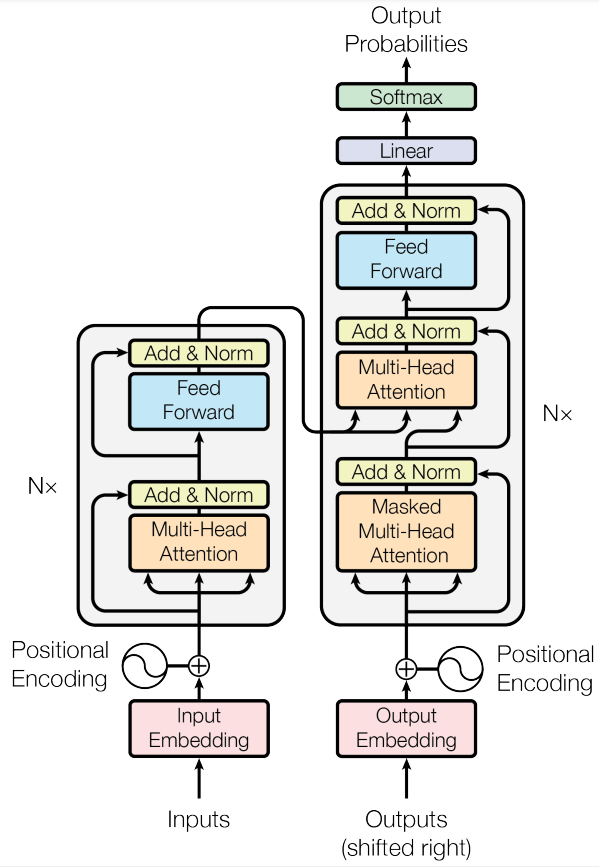
\includegraphics[width=6cm]{ressources/images/Transformer.png}
    \caption{transformer architecture from the original paper}
    \end{figure}
\subsection{Encoder}
The encoder takes an input sequence, and breaks it down into individual tokens (words or sub-words).
For each token an embedding vector is computed, which is a numerical representation of that token, capturing its semantic meaning.

A key component of the encoder is the self-attention mechanism. Self-attention enables the model to consider the entire sequence when encoding each token, allowing it to weigh the relevance of other tokens in the input sequence dynamically. For each token, the self-attention mechanism computes attention scores that determine the influence of all other tokens in the sequence. So the generated embedded vector for each token does not only represent the token alone but also its left and right contextual influence.


The encoder consists of multiple identical layers, or encoder blocks. Each encoder block contains two main sub-layers:

\begin{itemize}
    \item \textbf{Multi-Head Self-Attention Layer}: This sub-layer allows the model to attend to different parts of the sequence from multiple perspectives or "heads." Each head performs self-attention independently, and their outputs are concatenated and linearly transformed to provide a richer representation.

    \item \textbf{Feed-Forward Layer}: After the self-attention sub-layer, each token's representation is passed through a feed-forward neural network. This layer is a simple fully connected feed-forward network applied to each position (word) in the sequence independently and identically. It consists of two linear transformations with a ReLU activation in between, allowing the model to apply non-linear transformations and further refine the encoded representation.
\end{itemize}

Both sub-layers in the encoder block are followed by residual connections and layer normalization, which help in stabilizing the training and improving convergence.

\subsection{Decoder}
The decoder works quiet similar to the encoder and can be also be used for same tasks but with respect to loss of performance. It also uses multiple decoder blocks, similar to the encoder but has two additional sub-layers per block as compared to the encoder block. In the transformer's architecture the decoder's role is to generate the output sequence based on the encoded representation from the encoder (cross-attention). This is done auto-regressively, which means that the generated computed feature-vector, which holds information about the input sequence will be tranformed by the language modelling head mapping into the next probable following word, which then will be added to the input text and then get feeded back into the decoder. The most important difference to the encoder is the masked multi-head self-attention.

\begin{itemize}
    \item \textbf{Masked Multi-Head Self-Attention Layer}:
          Since the decoder cannot predict future words based on information not yet generated, it only attends uni-directional to the previously generated tokens in the output sequence. Therfor only the left context (for "LTR" text) is used and the right context is masked.
\end{itemize}





\section{BERT}
BERT (Bidirectional Encoder Representations from Transformers) is a  pre-trained language representation model introduced by Devlin et al. in 2019 (ref). Its based on the Transformer architecture from\dots but instead of using in contrast to using both, an encoder and a decoder as in the original transformer, BERT only utilizes the encoder component. Consequently, unlike other large language models (LLMs), BERT cannot predict new tokens and thus is not suitable for text generation. Instead, it still achieves state-of-the-art results in tasks such as text classification, sentiment analysis, and named entity recognition. The attention scores are computed using queries, keys, and values derived from the input embeddings.

\subsection{Embeddings}
The three matrices in BERT—token embeddings, segment embeddings, and positional embeddings are generated as part of the model's training process.

For each unique Token ID (i.e. for each of the 30,522 words and subwords in the BERT Tokenizer’s vocabulary), the BERT model contains an embedding that is trained to represent that specific token. The Embedding Layer within the model is responsible for mapping tokens to their corresponding embeddings.

Before a string of text is passed to the BERT model, the BERT Tokenizer is used to convert the input from a string into a list of integer Token IDs, where each ID directly maps to a word or part of a word in the original string. In addition to the Token Embeddings described so far, BERT also relies on Position Embeddings. While Token Embeddings are used to represent each possible word or subword that can be provided to the model, Position Embeddings represent the position of each token in the input sequence.

The final type of embedding used by BERT is the Token Type Embedding, also called the Segment Embedding in the original BERT Paper. One of the tasks that BERT was originally trained to solve was Next Sentence Prediction. That is, given two sentences A and B, BERT was trained to determine whether B logically follows A.\\

BERT introduces two pre-training objectives, the masked language model objective (MLM), and the next sentence prediction objective (NSP).


\begin{itemize}
    \item \textbf{Masked Language Modeling (MLM)}:
          15\% of the words in a sentence are randomly masked, and the model is trained to predict these masked words based on the context provided by the other words in the sentence. This enables BERT to learn bidirectional representations.

    \item \textbf{Next Sentence Prediction (NSP)}:
          To understand relationships between sentences, BERT is trained on pairs of sentences. Given two sentences, the model predicts whether the second sentence is the actual next sentence in the original text or a randomly chosen one. This task helps BERT capture the coherence and context between sentences.
\end{itemize}


\subsection{Fine-Tuning}
After pre-training on large text corpora, BERT can be fine-tuned on specific downstream tasks with relatively small amounts of data. Fine-tuning involves adjusting the pre-trained model weights slightly to better fit the target task. This approach leverages the robust pre-trained language representations and adapts them to the specific requirements of the task at hand.




\subsection{BERTScore}
BERTScore is an evaluation metric that utilizes the BERT model to compare texts more semantically than traditional metrics like BLEU. It leverages the contextualized embeddings provided by a pre-trained BERT model to assess the similarity between candidate and reference texts.\\

The process begins by inputting both candidate and reference texts into the BERT model, which generates contextualized embeddings for each token in both texts. For each token, the similarity between its embedding and every token embedding in the comparison text is calculated using cosine similarity
\begin{equation}
    \cos(\theta) = \frac{\mathbf{A} \cdot \mathbf{B}}{\|\mathbf{A}\| \|\mathbf{B}\|} = \frac{\sum_{i=1}^{n} \mathbf{A}_{i} \mathbf{B}_{i} }{\sqrt{\sum_{i=1}^{n} \mathbf{A}_{i}} \cdot \sqrt{\sum_{i=1}^{n} \mathbf{B}_{i}} }
\end{equation}
This results in a similarity matrix where each entry represents the cosine similarity between the embeddings of a pair of tokens (one from the candidate sentence and one from the reference sentence).\\


The metric is computed symmetrically as follows:\\

For each token embedding in the candidate sentence, find the maximum similarity score with any token embedding in the reference sentence, and average these scores across all tokens in the candidate sentence to obtain precision.\\

Similarly, for each token embedding in the reference sentence, find the maximum similarity score with any token embedding in the candidate sentence, and average these scores across all tokens in the reference sentence to obtain recall.

\[P_{BERT} = \frac{1}{|\hat{x}|} \sum_{\hat{x}_j\in \hat{x}} \max_{x_i \in x} x_i^T \hat{x_j} \]
\[R_{BERT} = \frac{1}{|x|} \sum_{x_i \in x} \max_{\hat{x}_j\in \hat{x}} x_i^T \hat{x_j} \]



Finally the $F_1$-score (an $F$-measure)
is computed as the harmonic mean of precision and recall and is providing a balanced measure that considers both the model's ability to capture relevant information and its accuracy in predicting new text equally.

\[F_{BERT} = 2\frac{P_{BERT}R_{BERT}}{P_{BERT} + R_{BERT}} \]

\section{BLEU-Score}

BLEU-Score is a different metric I use in my thesis for comparing texts. BLEU is not evaluating and comparing the semantic of the reference and candidate text but instead comparing similarity of vocabulary between them.

Let $\left\{y^{1}, y^{2}, ..., y^{N}\right\}$ be the words of the reference text and $\left\{\hat{y}^{1}, \hat{y}^{2}, ..., \hat{y}^{N}\right\}$


The first step is to create n-grams $\text{G}_n(y)$ for both texts. An n-gram is just a set of consecutive words of length n in a text.

\[
    \text{G}_n(y) = \left\{y_1, y_2, ..., y_k\right\}
\]

Next we define the function $\text{C}(s,y)$ that counts the appearances of s as a substring in y.
Now we can count n-grams of the candidate that appear in the reference text. We can compute the clipped precision by taking the minimum of the appearances of the n-gram in $y$ and $\hat{y}$ and then dividing by the amount of all occurences of n-grams in $\hat{y}$. Therefor candidates that have the same n-gram repeating over and over again don't get a higher precision score if the same n-gram does not appear in the reference text the same amount.

\[
    \text{p}_n(\hat{y} , y) = \frac{\sum_{s \in G_n(\hat{y})} \min(\text{C}(s,\hat{y}), \text{C}(s,y))}{\sum_{s \in G_n(\hat{y})} \text{C}(s,\hat{y})}
\]


Right now short candidate texts are more likely to get a good score although the reference text is much longer. Therefor we add a brevity penalty in order to give higher scores to texts that are closer or even longer to the reference texts real size.
\[
    \text{BP}(c, r) = \left\{\begin{array}{lr}
        1,               & \text{if } c > r    \\
        \ e^{(1 - r/c)}, & \text{if } c \leq r \\
    \end{array}\right\}
\]

Finally for BLEU-Score we combine the brevity penalty with the clipped precision of n-grams. We additionally add a distribution vector to weigh each $ \text{p}_n$ by $w_n$ in order to have the opportunity to give n-grams with different $n$ also a different impact on the overall result. Although in the end most BLEU-Scores just use a uniform distribution with $N = 4$ so that $w_n$ always stays $\frac{1}{4}$

\[\text{BLEU} = \text{BP}(c, r) \cdot \exp\left(\sum_{n=1}^{N}  \text{w}_n \cdot \ln(p_n)\right)\]



\chapter{Gathering of literature}
Unfortunately, there's barely any open-source collection of literature with 
characterizations available. Examples like "Romeo and Juliet," "Moby Dick," "Frankenstein," or "Alice's Adventures in Wonderland" are rare cases where enough fandom exists to create accessible and reviewed content. In most other instances, it seems too risky to use open-source literature, as these collections predominantly consist of less popular books with minimal fanbase and related content. Popular literature, with its larger online presence, results in more detailed and reviewed community-generated content, such as characterizations and summaries, which are valuable as reference points for my generated characterizations.\\

All of the books contained text decorations and structural elements such as chapters, sections, and page numbers, which remained present after converting the PDFs and text files and loading them into memory. These elements had to be manually filtered out before further processing, as they interfered with some of the techniques applied later.\\

During the process of using Wikidata, a free and open knowledge database, to query characters and filter personal descriptions from books, I discovered that many of these descriptions contain references to articles from Fandom.com, the world's most popular open-source wiki platform for fan-related content.\\

Initially, I planned to query Wikidata for all characters linked to Fandom articles to gather literature with the most comprehensive fandom articles. However, I realized that not all character descriptions in Wikidata include Fandom article links. Some character descriptions are missing Fandom article URLs, making it insufficient to rely solely on Wikidata for content. Additionally, there are instances of multiple articles linked to one character. Some articles are in different languages, while others are older versions or from different universes within the same saga. In most cases, I was able to chose to use the newest, longest English version but this was not always possible. For example, when fetching Dune character fandom articles, I had to manually sort out some characters. The Dune fandom includes characters from the "Dune Encyclopedia" and "Expanded Dune," as well as from the original "Dune" by Frank Herbert. This overlap made it problematic to compare information about the same character in different contexts, especially when relevant information might not be available across all contexts.\\


So in the end, I used multiple methods. First, I queried Wikidata to quickly obtain a large number of characters, then manually deleted duplicates and added additional characters with URLs by hand. Since readers of this thesis might not have access to all the non-open-source literature I used, I aimed to minimize the number of sources to make the results easier to replicate and verify. Ultimately, I was able to obtain character data for 800 characters from eight books in total. The results are linked in the appendix.



\begin{table}[h!]
  \centering
  \begin{tabular}{|l|c|}
  \hline
  \textbf{Book} & \textbf{Amount} \\
  \hline
  Harry Potter & 157 \\
  \hline
  Dune & 103  \\
  \hline
  Twilight & 72  \\
  \hline
  Alice's Adventures in Wonderland & 30 \\
  \hline
  The Lord of the Rings & 53 \\
  \hline
  The Hitchhiker's Guide to the Galaxy & 90 \\
  \hline
  The Hunger Games & 29 \\
  \hline
  \hline
  Total & 534 \\
  \hline
  \end{tabular}
  \caption{dataset of characters and their descriptions}
  \label{tab:example_table}
  \end{table}
...\\


Project Gutenberg and the Tell Me Again! Dataset...







\chapter{Experiments}

All my experiments have been conducted partially on my own computer but also on a remote server from the LT group at the University of Hamburg. This was mainly due to accessing a better GPU like the RTX A1000 NVIDEA for prompting LLMS and creating embeddings.


\section{Base Experiment}

For my first experiment, I formulated four prompts with slightly different wordings to observe how varying prompts affect the outcomes of the LLM. For each prompt, I tested two versions: one with additional passages from the literature providing information about the character, and one without such information, requiring the model to rely solely on its training data. ``[INST]'' and ``[\textbackslash INST]'' mark the start and end of each query instruction. ``\{character\}'' and ``\{book\}'' will be replaced with the real character name and book title. ``\{passages\}'' marks the spot where a collection of retrieved passages from the book for the given character that might help the Llama model with its characterizations will be passed into the prompt.\\



\begin{center}
    \begin{tabular}{|c|m{10cm}|}
        \hline
        Prompt        & Instruction                                                                                                                                             \\ [0.5ex]
        \hline\hline
        $\delta_{1}$  & "[INST]Write a summary about the character \{character\} in the book \{book\}.[/INST]"                                                                  \\
        \hline
        $\delta_{1}'$ & "[INST]Write a summary about the character \{character\} in the given text passages: \textbackslash n \{help\}[/INST]"                                  \\
        \hline\hline
        $\delta_{2}$  & "[INST]Write a summary in the style of a fandom article about the character \{character\} in the book \{book\}.[/INST]"                                 \\
        \hline
        $\delta_{2}'$ & "[INST]Write a summary in the style of a fandom article about the character \{character\} in the given text passages: \textbackslash n \{help\}[/INST]" \\
        \hline\hline
        $\delta_{3}$  & "[INST]Provide a concise overview of the character \{character\} from the book \{book\}.[/INST]"                                                        \\
        \hline
        $\delta_{3}'$ & "[INST]Provide a concise overview of the character \{character\} based on the following excerpts: \textbackslash n \{help\}[/INST]"                     \\
        \hline\hline
        $\delta_{4}$  & "[INST]rite sumary bout thee cara cter \{character\} of th book \{book\}.[/INST]"                                                                       \\
        \hline
        $\delta_{4}'$ & "[INST]rite sumary bout thee cara cter \{character\} bsed th fllowing excerpts: \textbackslash n \{help\}[/INST]"                                       \\ [1ex]
        \hline
    \end{tabular}
\end{center}



As you can see, $\delta_{2}$ is more specific, requesting the style of a fandom article, whereas $\delta_{3}$ is less precise, asking only for an overview without specifying a particular format. The last prompt is similar to $\delta_{1}$ but is intentionally faulty by missing characters.These different prompts are used to determine the overall effects of various prompt wordings and faulty instructions on the language model.



In this first experiment, I selected additional information from the book by filtering for every sentence in which the character's name occurred at least once. Since the number of tokens might exceed the maximum input size of the LLaMA model, I removed every $n$-th sentence, where $n$ is calculated in such a way that the query size fits perfectly.
Additionally, because characters are more likely to be introduced in the first sentences where they appear in the book, I added an additional cutoff $\alpha$. This cutoff represents the percentage of relevant sentences (with character name occurrences) to which every sentence with name occurence will be taken, so the rule of taking every $n$-th sentence only affects sentences after the cutoff. Overall the passage retrieval for this experiment $R_{base}$ works as follows. Let $S = \{s_i \mid 1 \leq i \leq k \}$ be the set of size $k$ which contains all relevant sentences containig the character and $l$ be the maximum inputsize of the Llama query. We first definde a function $S_{t}(a, b) = \{ s_{ti} \mid a \cdot k \leq ti \leq b \cdot k \}$, that enables a range selection of sentences with a lower and upper limit and a parameter $t$ for the stepsize. If we now choose our $n$ the right way 
\[n = \begin{cases} 
    \left\lfloor \frac{k - \alpha k}{l}\right\rfloor & \text{if } k - \alpha k > l\\
    1 & \text{otherwise}
\end{cases} \] we can write $R_{base}$ as \[R_{base} = S_{1}(0, \alpha) \cup S_{n} ( \alpha, 1) \].
I fed the prompts through the mixtral 7b model with quantized weights.
Quantization is a method used to decrease the computational and memory demands of running inference by using low-precision data types, such as 8-bit integers (int8), instead of the standard 32-bit floating-point (float32). Using fewer bits reduces the memory storage needed for the model, theoretically lowers energy consumption, and speeds up operations like matrix multiplication through integer arithmetic. This technique also enables models to run on embedded devices, which may only support integer data types. They are different types and levels of quantization and i started with the smallest $Q2_K$ (https://huggingface.co/ikawrakow/mixtral-instruct-8x7b-quantized-gguf) weights and therfor quickest responses. For the evaluation, I used BLEUScore and BERTScore to compare the results from the prompts against manually written articles from fandom.com.\\

% \begin{figure}
% \centering
% \begin{tikzpicture}
% \begin{axis}[
%     xlabel={F1},
%     ylabel={h},
%     legend pos=north west,
%     grid=both,
%     width=10cm, % Adjust width as needed
%     height=8cm % Adjust height as needed
% ]

% \addplot+[mark=none] table [x expr=\coordindex, y=F1, col sep=comma] {ressources/data/results.csv};


% \legend{P, R, F1, h}

% \legend{Data}
% \end{axis}
% \end{tikzpicture}
% \caption{Plot of F1 vs h}
% \label{fig:f1_vs_h}
% \end{figure}

% \begin{figure}
% \centering
% \begin{tikzpicture}
% \begin{axis}[
%     xlabel={F1},
%     ylabel={h},
%     legend pos=north west,
%     grid=both,
%     width=10cm, % Adjust width as needed
%     height=8cm % Adjust height as needed
% ]


% \addplot+[mark=none] table [x expr=\coordindex, y=wF1, col sep=comma] {ressources/data/results.csv};

% \legend{P, R, F1, h}

% \legend{Data}
% \end{axis}
% \end{tikzpicture}
% \caption{Plot of F1 vs h}
% \label{fig:f1_vs_h}
% \end{figure}

% \subsection{Results}
% \begin{figure}[H]
%     \centering
%     \begin{tikzpicture}
%         \begin{axis}[
%                 xlabel={F1},
%                 ylabel={h},
%                 legend pos=north west,
%                 grid=both,
%                 width=10cm, % Adjust width as needed
%                 height=8cm % Adjust height as needed
%             ]


%             \addplot+[mark=none] table [x expr=\coordindex, y=h, col sep=comma] {ressources/data/results.csv};

%             \legend{P, R, F1, h}

%             \legend{Data}
%         \end{axis}
%     \end{tikzpicture}
%     \caption{Plot of F1 vs h}
%     \label{fig:f1_vs_h}
% \end{figure}

\subsection{Results}
% \begin{figure}[H]
%     \centering
%     \makebox[\textwidth][c]{
%         \begin{minipage}{1.1\textwidth}
%             \begin{subfigure}[b]{0.45\textwidth}
%                 \centering
%                 \begin{tikzpicture}
%                     \begin{axis}[
%                             x tick label style={
%                                     /pgf/number format/1000 sep=},
%                             xlabel=BLEUScore,
%                             ylabel=Amount,
%                             enlargelimits=0.05,
%                             legend style={at={(1.0,-0.2)},
%                                     anchor=north,legend columns=-1},
%                             ybar interval=0.7,
%                         ]
%                         \addplot
%                         coordinates {(0.0,1) (1.4,288) (2.8,50) (4.3,15) (5.7,6) (7.2,1) (8.6,1) (11.5,1) };
%                         \addplot
%                         coordinates {(0.0,0) (1.4,266) (2.8,57) (4.3,24) (5.7,8) (7.2,7) (8.6,2) (11.5,0) };

%                         \legend{$\delta'$,$\delta$}
%                     \end{axis}
%                 \end{tikzpicture}
%                 \label{fig:enter-label}
%             \end{subfigure}
%             \hfill
%             \begin{subfigure}[b]{0.45\textwidth}
%                 \centering
%                 \begin{tikzpicture}
%                     \begin{axis}[
%                             x tick label style={
%                                     /pgf/number format/1000 sep=},
%                             xlabel=BERTScore,
%                             enlargelimits=0.05,
%                             legend style={at={(1.0,-0.2)},
%                                     anchor=north,legend columns=-1},
%                             ybar interval=0.7,
%                         ]
%                         \addplot
%                         coordinates {(0.38,0) (0.43,4) (0.47,46) (0.52,157) (0.56,119)
%                                 (0.61,31) (0.65,0) };
%                         \addplot
%                         coordinates {(0.38,0) (0.43,0) (0.47,11) (0.52,90) (0.56,197)
%                                 (0.61,60) (0.65,0) };

%                         \legend{$\delta'$,$\delta$}
%                     \end{axis}
%                 \end{tikzpicture}
%                 \label{fig:enter-label}
%             \end{subfigure}
%         \end{minipage}
%     }
%     \caption{Distribution of BERTScore and Blue-Metric without ($\delta$) and with passage retrieval ($\delta'$) in bins}
% \end{figure}













% ScatterPLOTS




\begin{figure}[H]
    \centering
    \makebox[\textwidth][c]{
        \begin{minipage}{1.1\textwidth}
            \centering
            \begin{subfigure}[b]{0.45\textwidth}
                \centering
                \begin{tikzpicture}
                    \begin{axis}[
                            enlargelimits=false,
                            title={Prompt 1},
                            xlabel={$BLEU(\delta)$},
                            ylabel={$BLEU(\delta')$},
                            xmin=0.35, xmax=0.65,
                            ymin=0.35, ymax=0.65,
                            xtick distance=0.1, ytick distance=0.1
                        ]
                        \addplot[color=black, thick, dotted] {x};
                        \addplot+[
                            color=blue,
                            only marks,
                            mark=o,
                            mark size=1.0pt]
                        table [col sep=comma, x=F1, y=wF1] {ressources/data/results.csv};
                    \end{axis}
                \end{tikzpicture}
                \label{fig:prompt1}
            \end{subfigure}
            \hfill
            \begin{subfigure}[b]{0.45\textwidth}
                \centering
                \begin{tikzpicture}
                    \begin{axis}[
                            enlargelimits=false,
                            title={Prompt 2},
                            xlabel={$BLEU(\delta)$},
                            xmin=0.35, xmax=0.65,
                            ymin=0.35, ymax=0.65,
                            xtick distance=0.1, ytick distance=0.1
                        ]
                        \addplot[color=black, thick, dotted] {x};
                        \addplot+[
                            color=blue,
                            only marks,
                            mark=o,
                            mark size=1.0pt]
                        table [col sep=comma, x=F1, y=wF1] {ressources/data/results2.csv};
                    \end{axis}
                \end{tikzpicture}
                \label{fig:prompt2}
            \end{subfigure}
            \vspace{0.5cm}
            \begin{subfigure}[b]{0.45\textwidth}
                \centering
                \begin{tikzpicture}
                    \begin{axis}[
                            enlargelimits=false,
                            title={Prompt 3},
                            xlabel={$BLEU(\delta)$},
                            ylabel={$BLEU(\delta')$},
                            xmin=0.35, xmax=0.65,
                            ymin=0.35, ymax=0.65,
                            xtick distance=0.1, ytick distance=0.1
                        ]
                        \addplot[color=black, thick, dotted, domain=0:16] {x};
                        \addplot+[
                            color=blue,
                            only marks,
                            mark=o,
                            mark size=1.0pt]
                        table [col sep=comma, x=F1, y=wF1] {ressources/data/results3.csv};
                    \end{axis}
                \end{tikzpicture}
                \label{fig:prompt3}
            \end{subfigure}
            \hfill
            \begin{subfigure}[b]{0.45\textwidth}
                \centering
                \begin{tikzpicture}
                    \begin{axis}[
                            enlargelimits=false,
                            title={Prompt 4},
                            xlabel={$BLEU(\delta)$},
                            xmin=0.35, xmax=0.65,
                            ymin=0.35, ymax=0.65,
                            xtick distance=0.1, ytick distance=0.1
                        ]
                        \addplot[color=black, thick, dotted, domain=0:16] {x};
                        \addplot+[
                            color=blue,
                            only marks,
                            mark=o,
                            mark size=1.0pt]
                        table [col sep=comma, x=F1, y=wF1] {ressources/data/results4.csv};
                    \end{axis}
                \end{tikzpicture}
                \label{fig:prompt4}
            \end{subfigure}
        \end{minipage}
    }
    \caption{Blue-Metric of Zero-Shot Characterizations generated with Llama without ($\delta$) and with passage retrieval ($\delta'$) from the literature}
\end{figure}

\begin{figure}[H]
    \centering
    \makebox[\textwidth][c]{
        \begin{minipage}{1.1\textwidth}
            \begin{subfigure}[b]{0.45\textwidth}
                \centering
                \begin{tikzpicture}
                    \begin{axis}[
                            enlargelimits=false,
                            title={Prompt 1},
                            xlabel={$BERT(\delta)$},
                            ylabel={$BERT(\delta')$},
                            xmin=0, xmax=16,
                            ymin=0, ymax=16
                        ]
                        \addplot[color=black, thick, dotted, domain=0:16] {x};
                        \addplot+[
                            color=blue,
                            only marks,
                            mark=o,
                            mark size=1.0pt]
                        table [col sep=comma, x=h, y=wh]
                            {ressources/data/results.csv};
                    \end{axis}
                \end{tikzpicture}
                % \caption{Blue-Metric of Characterizations generated with Llama prompt 1 with and without additional textpassages from the literatur}
                \label{fig:enter-label}
            \end{subfigure}
            \hfill
            \begin{subfigure}[b]{0.45\textwidth}
                \centering
                \begin{tikzpicture}
                    \begin{axis}[
                            enlargelimits=false,
                            title={Prompt 2},
                            xlabel={$BERT(\delta)$},
                            % ylabel={prompt with additional textpassages},
                            xmin=0, xmax=16,
                            ymin=0, ymax=16
                        ]
                        \addplot[color=black, thick, dotted, domain=0:16] {x};
                        \addplot+[
                            color=blue,
                            only marks,
                            mark=o,
                            mark size=1.0pt]
                        table [col sep=comma, x=h, y=wh]
                            {ressources/data/results.csv};
                    \end{axis}
                \end{tikzpicture}
                % \caption{Blue-Metric of Characterizations generated with Llama prompt 1 with and without additional textpassages from the literatur}
                \label{fig:enter-label}
            \end{subfigure}
            \vspace{0.5cm}
            \begin{subfigure}[b]{0.45\textwidth}
                \centering
                \begin{tikzpicture}
                    \begin{axis}[
                            enlargelimits=false,
                            title={Prompt 3},
                            xlabel={$BERT(\delta)$},
                            ylabel={$BERT(\delta')$},
                            xmin=0, xmax=16,
                            ymin=0, ymax=16
                        ]
                        \addplot[color=black, thick, dotted, domain=0:16] {x};
                        \addplot+[
                            color=blue,
                            only marks,
                            mark=o,
                            mark size=1.0pt]
                        table [col sep=comma, x=h, y=wh]
                            {ressources/data/results.csv};
                    \end{axis}
                \end{tikzpicture}
                % \caption{BERTScore of Characterizations generated with Llama prompt 1 with and without additional textpassages from the literatur}
                \label{fig:enter-label}
            \end{subfigure}
            \hfill
            \begin{subfigure}[b]{0.45\textwidth}
                \centering
                \begin{tikzpicture}
                    \begin{axis}[
                            enlargelimits=false,
                            title={Prompt 4},
                            xlabel={$BERT(\delta)$},
                            % ylabel={prompt with additional textpassages},
                            xmin=0, xmax=16,
                            ymin=0, ymax=16
                        ]
                        \addplot[color=black, thick, dotted, domain=0:16] {x};
                        \addplot+[
                            color=blue,
                            only marks,
                            mark=o,
                            mark size=1.0pt]
                        table [col sep=comma, x=h, y=wh]
                            {ressources/data/results.csv};
                    \end{axis}
                \end{tikzpicture}
                % \caption{BERTScore of Characterizations generated with Llama prompt 1 with and without additional textpassages from the literatur}
                \label{fig:enter-label}
            \end{subfigure}
        \end{minipage}
    }
    \caption{BERTScore of Zero-Shot Characterizations generated with Llama without ($\delta$) and with passage retrieval ($\delta'$) from the literatur}
\end{figure}



%Other




\begin{figure}[H]
    \centering
    \begin{subfigure}[b]{\textwidth}
        \centering
        \begin{tikzpicture}
            \pgfplotstableread[col sep=comma]{ressources/data/boxplot.csv}\csvdata
            \pgfplotstabletranspose\datatransposed{\csvdata}
            \begin{axis}[
                    boxplot/draw direction = y,
                    axis x line* = bottom,
                    axis y line = left,
                    enlarge y limits,
                    ymajorgrids,
                    cycle list={{blue}},
                    xtick = {1,2,3,4,5,6,7,8},
                    xticklabel style = {align=center, font=\small},
                    xticklabels = {$\delta_{1}$, $\delta_{1}'$, $\delta_{2}$, $\delta_{2}'$, $\delta_{3}$, $\delta_{3}'$, $\delta_{4}$, $\delta_{4}'$},
                    xtick style = {draw=none},
                    ylabel = {$BLEU$}
                ]
                \foreach \n in {1,...,8} {
                        \addplot+[boxplot, draw=black] table[y index=\n] {\datatransposed};
                    }
            \end{axis}
        \end{tikzpicture}
        \label{fig:boxplot}
    \end{subfigure}
    \hfill
    \vspace{1cm}
    \hfill
    \begin{subfigure}[b]{\textwidth}
        \centering
        \begin{tikzpicture}
            \begin{groupplot}[
                    group style={
                            group size=1 by 2,
                            vertical sep=0pt
                        },
                    boxplot/draw direction = y,
                    enlarge y limits,
                    ymajorgrids,
                    cycle list={{blue}},
                    xmin=0,
                    xmax=9,
                    height=10cm,
                    width=10cm
                ]
                \nextgroupplot[
                    hide x axis,
                    axis y line=left,
                    axis y discontinuity=parallel,
                    ymin=7,
                    ymax=18,
                    height=3.5cm,
                    y label style={at={(axis description cs:-0.1,.1)},rotate=0,anchor=south},
                    ylabel = ${BERT}$
                ]

                \addplot+[
                    boxplot prepared from table={
                            table=\csvdata,
                            row=0, % 0-based index
                            lower whisker=lw,
                            upper whisker=uw,
                            lower quartile=lq,
                            upper quartile=uq,
                            median=med
                        }, boxplot prepared,   draw=black
                ]
                coordinates {};

                \addplot+[
                    boxplot prepared from table={
                            table=\csvdata,
                            row=1, % 0-based index
                            lower whisker=lw,
                            upper whisker=uw,
                            lower quartile=lq,
                            upper quartile=uq,
                            median=med
                        }, boxplot prepared,   draw=black
                ]
                coordinates {};

                \addplot+[
                    boxplot prepared from table={
                            table=\csvdata,
                            row=2, % 0-based index
                            lower whisker=lw,
                            upper whisker=uw,
                            lower quartile=lq,
                            upper quartile=uq,
                            median=med
                        }, boxplot prepared,   draw=black
                ]
                coordinates {};
                \addplot+[
                    boxplot prepared from table={
                            table=\csvdata,
                            row=3, % 0-based index
                            lower whisker=lw,
                            upper whisker=uw,
                            lower quartile=lq,
                            upper quartile=uq,
                            median=med
                        }, boxplot prepared,   draw=black
                ]
                coordinates {};

                \addplot+[
                    boxplot prepared from table={
                            table=\csvdata,
                            row=4, % 0-based index
                            lower whisker=lw,
                            upper whisker=uw,
                            lower quartile=lq,
                            upper quartile=uq,
                            median=med
                        }, boxplot prepared,   draw=black
                ]
                coordinates {};

                \addplot+[
                    boxplot prepared from table={
                            table=\csvdata,
                            row=5, % 0-based index
                            lower whisker=lw,
                            upper whisker=uw,
                            lower quartile=lq,
                            upper quartile=uq,
                            median=med
                        }, boxplot prepared,   draw=black
                ]
                coordinates {};

                \addplot+[
                    boxplot prepared from table={
                            table=\csvdata,
                            row=6, % 0-based index
                            lower whisker=lw,
                            upper whisker=uw,
                            lower quartile=lq,
                            upper quartile=uq,
                            median=med
                        }, boxplot prepared,   draw=black
                ]
                coordinates {};

                \addplot+[
                    boxplot prepared from table={
                            table=\csvdata,
                            row=7, % 0-based index
                            lower whisker=lw,
                            upper whisker=uw,
                            lower quartile=lq,
                            upper quartile=uq,
                            median=med
                        }, boxplot prepared,   draw=black
                ]
                coordinates {};





                \nextgroupplot[
                    xtick = {1,2,3,4,5,6,7,8},
                    xticklabel style = {align=center, font=\small},
                    xticklabels = {$\delta_{1}$, $\delta_{1}'$, $\delta_{2}$, $\delta_{2}'$, $\delta_{3}$, $\delta_{3}'$, $\delta_{4}$, $\delta_{4}'$},
                    xtick style = {draw=none},
                    axis x line* = bottom,
                    axis y line = left,
                    ymin=0,
                    ymax=2,
                    height=3.5cm
                ]

                \addplot+[
                    boxplot prepared from table={
                            table=\csvdata,
                            row=0, % 0-based index
                            lower whisker=lw,
                            upper whisker=uw,
                            lower quartile=lq,
                            upper quartile=uq,
                            median=med
                        }, boxplot prepared,   draw=black
                ]
                coordinates {};

                \addplot+[
                    boxplot prepared from table={
                            table=\csvdata,
                            row=1, % 0-based index
                            lower whisker=lw,
                            upper whisker=uw,
                            lower quartile=lq,
                            upper quartile=uq,
                            median=med
                        }, boxplot prepared,   draw=black
                ]
                coordinates {};

                \addplot+[
                    boxplot prepared from table={
                            table=\csvdata,
                            row=2, % 0-based index
                            lower whisker=lw,
                            upper whisker=uw,
                            lower quartile=lq,
                            upper quartile=uq,
                            median=med
                        }, boxplot prepared,   draw=black
                ]
                coordinates {};
                \addplot+[
                    boxplot prepared from table={
                            table=\csvdata,
                            row=3, % 0-based index
                            lower whisker=lw,
                            upper whisker=uw,
                            lower quartile=lq,
                            upper quartile=uq,
                            median=med
                        }, boxplot prepared,   draw=black
                ]
                coordinates {};

                \addplot+[
                    boxplot prepared from table={
                            table=\csvdata,
                            row=4, % 0-based index
                            lower whisker=lw,
                            upper whisker=uw,
                            lower quartile=lq,
                            upper quartile=uq,
                            median=med
                        }, boxplot prepared,   draw=black
                ]
                coordinates {};

                \addplot+[
                    boxplot prepared from table={
                            table=\csvdata,
                            row=5, % 0-based index
                            lower whisker=lw,
                            upper whisker=uw,
                            lower quartile=lq,
                            upper quartile=uq,
                            median=med
                        }, boxplot prepared,   draw=black
                ]
                coordinates {};

                \addplot+[
                    boxplot prepared from table={
                            table=\csvdata,
                            row=6, % 0-based index
                            lower whisker=lw,
                            upper whisker=uw,
                            lower quartile=lq,
                            upper quartile=uq,
                            median=med
                        }, boxplot prepared,   draw=black
                ]
                coordinates {};

                \addplot+[
                    boxplot prepared from table={
                            table=\csvdata,
                            row=7, % 0-based index
                            lower whisker=lw,
                            upper whisker=uw,
                            lower quartile=lq,
                            upper quartile=uq,
                            median=med
                        }, boxplot prepared,   draw=black
                ]
                coordinates {};


            \end{groupplot}
        \end{tikzpicture}

        \label{fig:boxplot}
    \end{subfigure}
    \vspace{1cm}
    \caption{Boxplots of BLEU- and BERTScores for every prompt ($\delta_{1}, \delta_{1}', \delta_{2},...,\delta_{4}'$)}
\end{figure}



\subsection{Analysis}
Obviously the method of passage retrieval used for this experiment isn't ideal, as regularly eliminating sentences could omit important context, also at this stage, the process of fetching fandom articles wasn't complete, resulting in a dataset with some duplicates and missing characterizations. Despite these limitations, the data is still sufficient to show two important aspects of the data. First, the results with passage retrieval are at least as good as, or already slightly better than, those without. Second, the results vary only slightly across the four different prompts. Befor we investigate that further lets have an more detailed look at the results.\\

As we can see, the BLEU scores of each prompt mostly improve after passage retrieval. Although the maximum values of $\delta_{1}$ and $\delta_{2}$ have decreased slightly in $\delta_{1}'$ and $\delta_{2}'$, the minimum values, Q1, and Q3 have significantly increased, as observed in the box plots. For both $\delta_{3}$ and $\delta_{4}$, every box plot quartile has improved.\\

For BERTScore, the improvement isn't quite as visible. In fact, the upper quartiles have a lower maximum after passage retrieval, but Q1-Q3 has improved slightly for every prompt. Consequently, the results are more compact. Some outliers close to the maximum in Q4 might score so high prior to passage retrieval due to Llama being trained on similar information to the fandom articles. Especially when generating summaries for main characters, Llama might already have a great knowledge base for that character, and relying solely on the additional passed sentences might therefore be hindering in generating a good characterization.\\

In summary, semantically, the results have only improved slightly and the different wordings in the prompts definately have an influence on the results average and variance (ref figure).



\newpage
\section{Selected Embedded chunks}

We will now continue with prompt 1 from the base experiment since it had the highest results in both metrics. We will now improve on the method for passage retrieval.
\chapter{Conclusion}

\section{summary}
\section{future work}
For me, what comes first to mind when it comes to future work is how annoying and extensive time i had to put into scraping single pdfs. Every author has a different way to structure their book with different placements for pagenumbers, chapternumbers and -names which makes it really hard to find the right way to scrape them all efficiently. But plenty and clean data is so important when it is the bases for almost everything that follows up. Therefore i would condone to create the amount of literatur and characters and even improve on the already so carefully filtered data.
There is a second part to the mentioned data filtering which also leaves room to improve on which are the human-written fandom articles from fandom.com. Since some of them are so long since they contain so much detail i had to cut them to a specific paragraph. Take whole???

More evaluation methods

Since LLMs will continue to improve and might also increase their maximum input size to a point where maybe the input size will easily handle any single book, the task might shift to 

\section{note of thanks}
I would like to extend my heartfelt gratitude to all those who have knowingly or unknowingly supported me throughout the completion of this master's thesis.

First and foremost, to my advisor, Hans Ole Hatzel, for his unwavering guidance, invaluable insights, and constant encouragement. Your expertise and patience have been instrumental in shaping this research.

I would also like to thank my family and friends, whose love, support, and understanding throughout this semester provided me with both motivation and inspiration.


Finally, I am grateful to all those, named and unnamed, who have directly or indirectly contributed to this thesis. Your support has been invaluable, and I am deeply thankful for your contributions.

\printbibliography
\chapter{Appendix}
\textit{In this section I will link my repositories containing all my scripts and data that I created and collected during my thesis.}
\cleardoublepage

% VERZEICHNISSE (Abbildungen, Tabellen)
% Literatur 
%\nocite{wiki:wissarbeit}

\cleardoublepage

% ERKLÄRUNG
\chapter*{Eidesstattliche Versicherung}
\thispagestyle{empty}
\addcontentsline{toc}{chapter}{Eidesstattliche Versicherung}

Hiermit versichere ich an Eides statt, dass ich die vorliegende Arbeit selbstständig und ohne fremde Hilfe angefertigt und mich anderer als der im beigefügten Verzeichnis angegebenen Hilfsmittel nicht bedient habe.
Alle Stellen, die wörtlich oder sinngemäß aus Veröffentlichungen entnommen wurden, sind als solche kenntlich gemacht. 
Ich versichere weiterhin, dass ich die Arbeit vorher nicht in einem anderen Prüfungsverfahren eingereicht habe und die eingereichte schriftliche Fassung der auf dem elektronischen Speichermedium entspricht.

\noindent Ich bin mit einer Einstellung in den Bestand der Bibliothek des Fachbereiches einverstanden.

\vspace{2cm} 

\noindent Hamburg, den \uline{~~~~~~~~~~~~~~~~~~~~}~~~~~Unterschrift: \uline{~~~~~~~~~~~~~~~~~~~~~~~~~~~~~~~~~~~~~~~~~~~~~~~~~~} 

    
\end{document}